\chapter{Targeted Estimator}
\label{ch-targeted-est}

\newcommand{\dpsi}[0]{\nabla\Psi}
\newcommand{\hatl}[0]{\HAT{\call}}

This chapter is based on Refs.\cite{tlride} and  \cite{hoff}.

Targeted Estimator (TE) theory  addresses
the following concerns.
Suppose $\Psi[P]$ is an estimator that depends on the full probability distribution $P$ of a fixed bayesian network.
$\Psi[P]$ is a functional (i.e., a function of a function) of $P$. If $P$ is perturbed by a small amount $\delta P$, we get $\Psi[P+\delta P]$. $\Psi[P + \delta P]$ can be expanded in powers of $\delta P$.
The term linear  in $\delta P$ defines the \qt{influence function}; it
also defines the \qt{functional derivative}  of $\Psi$ with respect to $P$
. {\it Why are influence functions useful?}
 The influence function measures,
 to first order in $\delta P$, how the estimator $\Psi$ responds to a perturbation
 $\delta P$ in $P$. In general, $\Psi$ does not have to be a counterfactual estimator, but it might be one, like an estimator of ATE, or PNS or whatever.
{\it So what is this good for?} It is a way of generating linear
\qt{targeted} estimators
that are less noisy
and converge more quickly. It measures the sensitivity of an estimator to perturbations in $P$. It does not, however, measure sensitivity to changes in the DAG (the DAG is fixed throughout). And it does not generate new estimands.

The goal of TE and
the strategy one uses to achieve it, is
explained more precisely in the next section.




\section{Goal, Strategy, and Rationale of TE theory}


Let $\rvb = (\rvb_1, \rvb_2, \ldots, \rvb_{n})$ denote
the $n$ nodes of a Bayesian Network, and let $P_\rvb(b)$ for $b\in val(\rvb)$
denote the full probability distribution of the bnet.

 Consider a population $\Sigma$ of
 individuals $\s\in \Sigma$ with $N=|\Sigma|$.
 The {\bf empirical probability distribution}
 $P_N:val(\rvb) \rarrow [0,1]$ for this bnet is defined by

\beq
P_N(b) = \frac{1}{N}\sum_\s\delta(b, b_\s)
\eeq

\beq
\sum_b P_N(b)f(b)=
\frac{1}{N}\sum_\s f(b_\s)
\eeq
As $N\rarrow \infty$, $P_N(b)$ tends
to the probability distribution $P_\rvb(b)$
of the bnet.
\begin{figure}[h!]
$$
\xymatrix{
&\rvx_2\ar[ddl]\ar[ddr]
\\
\ul{\xi}_1\ar[r]
&\rvx_1\ar[dr]
&\ul{\xi}_2
\\
\rvd\ar[rr]\ar[u]\ar[rru]
&
&\rvy\ar[u]
}
$$
\caption{Example of bnet considered in TE
theory.}
\label{fig-targeted-bnet}
\end{figure}

Let $\rvb=(\rvX, \ul{\xi})$ and
$\rvX=(\rvd, \rvx,\rvy)$,
where
node $\rvd\in\bool$ denotes a decision to treat a patient,
node $\rvy\in \bool$ denotes the treatment outcome,
multi-node $\rvx$ denotes the covariates
that are good controls, and multi-node $\ul{\xi}$ denotes
the covariates that we don't want to control.
See Fig.\ref{fig-targeted-bnet}
for an example of a bnet that fits this description.


The curve-fit $\haty$ of $y$
is a function $\haty:val(\rvd)\times val(\rvx)\rarrow \RR$
that minimizes the {\bf loss (a.k.a. loss functional)} $\call$
given by


\beq
\call[P, \haty]= \sum_X P(X) \hatl[y, \haty(d,x)]^2
\;,
\eeq
where $\hatl(a,b)$, the {\bf loss
curve-fit}, is a
non-negative function
that vanishes when $a=b$.
The function $\hatl$ is designed
to minimize a particular kind of error.
In this chapter, the $\hatl$
is designed to reduce ATE error.


The estimate
 $\Psi[P, \haty]$ for the curve-fit $\haty$
is defined by

\beq
\Psi[P, \haty] =\sum_X P(X)\haty(d,x)
\eeq

Unfortunately, the words \qt{estimator}
and \qt{estimate} are often used
interchangeably. See Section
\ref{sec-estimand}.
In this chapter, we use $(\haty, \Psi)$
for our (estimator, estimate) pair,
and refer to estimators as curve-fits.


Let
\beq
\delta P(X)=
P(X)-P_{in}(X)
\eeq
where $P, P_{in}:val(\rvX)\rarrow [0,1]$ are
probability distributions.

Define $\delta\haty(X)$ by

\beq
\delta\haty(X)= \frac{\haty(d,x) \delta P(X)}{P(X)}
\eeq
Hence

\beq
P(X)\delta\haty(X) = \haty(d,x)\delta P(X)
\eeq
Since $\Psi[P, \haty]$
is linear in $P$ and $\haty$,
it follows that

\beq
\Psi[P, \haty + \delta\haty]=
\Psi[P + \delta P, \haty]
\eeq


Suppose $P_{in++}$ satisfies


\beq
P_{in++}= \argmin_{P_{in}}\call[P_{in}, \haty]
\eeq
and

\beq
\lim_{N\rarrow \infty}
\Psi[P_N, \haty + \delta\haty]=
\lim_{N\rarrow \infty}
\Psi[\underbrace{P_N+\delta P}_{P_{in++}}, \haty]
=
\lim_{N\rarrow \infty}
\Psi[P_N, \haty]
\label{eq-tar-limit}
\;.
\eeq
Eq.(\ref{eq-tar-limit}) is illustrated in
Fig.\ref{fig-targeted-p-psi-plot.png}.

The goal of TE theory
is to find, given a curve-fit $\haty$,
a new curve-fit $\haty +\delta \haty$
so that the
estimate $\Psi[P_N, \haty+\delta \haty]$
has better behavior as $N\rarrow \infty$ than
$\Psi[P_N, \haty]$ (i.e., converges faster,
has smaller bias and variance).


\begin{figure}[h!]
\centering
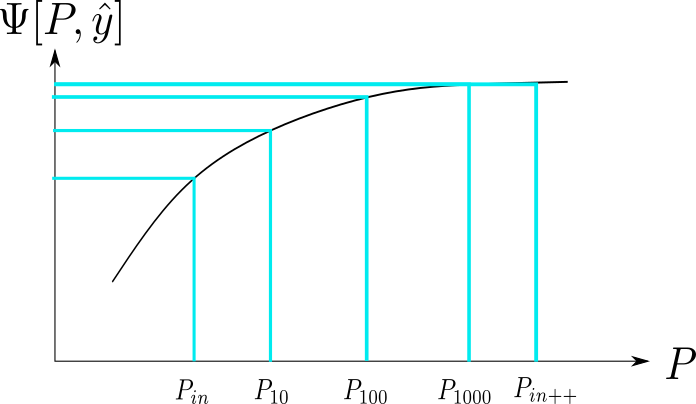
\includegraphics[width=3.5in]
{targeted-est/targeted-p-psi-plot.png}
\caption{
Plot of $\Psi[P, \haty]\in \RR$ versus $P$
at fixed $\haty$.
In reality, the $P$ are not real numbers but
functions.
}
\label{fig-targeted-p-psi-plot.png}
\end{figure}


\section{Functional Calculus}

Define
the Hilbert space of square integrable functions over $\rvX\in val(\rvX)$
by

\beq
\calh_\rvX =\{h: (h:val(\rvX)\rarrow \RR) \text{ and }
\sum_{ X\in S_ \rvX}[h(X)]^2 <\infty\}
\eeq
For any $f,g\in \calh_\rvX$,
define the dot product (a.k.a. inner product)
of $f$ and $g$ by

\beq
f\cdot g = \sum_X f(X) g(X)
\eeq
and the norm

\beq
\norm{f}_P= \sqrt{\sum_X [f(X)]^2}
\;.
\eeq

Suppose $P:val(\rvX)\rarrow [0,1]$
is a probability distribution.
Note that $P\in\calh_\rvX$.
For any $f,g\in\calh_\rvX$,
define the $P$ expected value by

\beq
\av{f}_P = P\cdot f
\eeq
and the $P$ covariance by
\beq
\av{f,g}_P =
\av{fg}_P - \av{f}_P\av{g}_P
\eeq

Suppose $\Psi[\eta]\in\RR$
is a real valued function
that depends on a function $\eta\in \calh_\rvX$.
$\Psi[\eta]$ is said to be a {\bf functional} of $\eta$.
Define the
{\bf functional derivative or gradient }\footnote{
Functional derivatives are commonly used in Physics
especially in Quantum Field Theory.
See Ref.\cite{wiki-func-deri} for more
information about them.}
of $\Psi[\eta]$ with respect to $\eta$, as follows


\beq
\frac{\delta \Psi[\eta]}
{\delta \eta(a)}=
\lim_{\eps\rarrow 0}
\frac{\Psi[\eta(x)+\eps\frac{\delta(x,a)}{\Delta x}] - \Psi[\eta(x)]}
{\eps}
\eeq
where $\delta(x,a)$ is the Kronecker delta function.
For example,
\beq
\frac{\delta}
{\delta \eta(a)}
\sum_x \Delta x\; \eta(x) h(x)
=
\sum_x \Delta x \frac{\delta(x,a)}{\Delta x} h(x)
=
h(a)
\eeq
 Let
$\delta(x-a)$ denote the Dirac delta function. If we replace
$\frac{\delta(x,a)}{\Delta x}\rarrow\delta(x-a)$
and $\sum_x \Delta x\rarrow \int dx$, we go
from the discrete to the continuous version
of the functional derivative.

\beq
\sum_x \Delta x \frac{\delta(x, a)}{\Delta x}
\rarrow \int dx\, \delta(x-a)
\eeq

In this chapter, we will use only the discrete version.
The $\Delta x$ in the numerator
and the one in the denominator, always cancel
each other when we go from discrete
to continuous, so we can
set
$\Delta x=1$ with impunity.



We will also use the notation

\beq
\dpsi[\eta](a)=
\frac{\delta \Psi[\eta]}
{\delta \eta(a)}
\;.
\eeq

Suppose $\eta, \eta_0\in \calh_\rvX$. Define the
{\bf functional Taylor expansion} of $\Psi[\eta]$
at $\eta_0$, as follows:

\beq
\Psi[\eta]=
\Psi[\eta_0]
+ \sum_x
\left[
\frac{\delta \Psi[\eta]}
{\delta \eta(x)}\right]_{\eta=\eta_0}
\delta\eta(x)
+
\frac{1}{2!}
\sum_{x,x'}
\left[
\frac{\delta^2 \Psi[\eta]}
{\delta\eta(x)\delta\eta(x') }\right]_{\eta=\eta_0}
\delta\eta(x)\delta\eta(x')
+
\cdots
\eeq
where we abbreviate
$ \eta =\eta(x)$,
$\eta_0=\eta_0(x)$ and $\delta \eta(x) = \eta(x)-\eta_0(x)$.



Define the
{\bf functional directional derivative of $\Psi[\eta]$ in
the $h\in \calh_\rvX$
direction}
by $h\cdot\frac{\delta \Psi[\eta]}{\delta \eta}$.
If one compares functional calculus with vector calculus, we see that
$\frac{\delta \Psi[\eta]}{\delta \eta}$ corresponds to a gradient
$\nabla f(\vecx)$ and
$h\cdot \frac{\delta \Psi[\eta]}{\delta \eta}$
corresponds to a directional derivative
$\vecd\cdot \nabla f(\vecx)$.
For $|\vecd|<<1$, $\vecd\cdot \nabla f(\vecx)$ approximates
the change
in $f(\vecx)$ when $\vecx$ moves from $\vecx$ to $\vecx+\vecd$


\section{Linear Approximation of $\Psi[P_N]$}



Consider probability
distributions $P, P_{in}:val(\rvX)\rarrow [0,1]$.
The {\bf linear approximation (a.k.a.
one-step-approximation)}
to the Taylor expansion of $\Psi[P]$ at
$P_{in}$ is given by

\beq
\underbrace{\Psi[P] - \Psi[P_{in}]}_{\delta \Psi[P,P_{in}]}]=
\sum_X
\underbrace{\left[\frac{\delta\Psi[P]}{\delta P(X)}
\right]_{P=P_{in}}
}_{\dpsi[P_{in}](X)}
\
\underbrace{\delta P(X)}_{P(X)-P_{in}(X)}
+
\calr[P, P_{in}]
\label{eq-1st-order-psi}
\eeq
If we set

\beq
\dpsi_{in} = \av{\dpsi[P_{in}]}_{P_{in}}
\;,
\eeq
then Eq.(\ref{eq-1st-order-psi}) becomes

\beqa
\delta\Psi[P,P_{in}]&=&
\sum_X P(X)
\underbrace{
\{\dpsi[P_{in}](X) - \dpsi_{in}\}
}_{\lam(X)}
+
\calr[P, P_{in}]
\eeqa
$\lam(X)$  is called the {\bf efficient influence curve (EIF)}.

Recall the Cauchy-Schwartz (CS) inequality for $\vec{a}, \vec{b}\in\RR^n$:

\beq
\vec{a}\cdot\vec{b} =|\vec{a}||\vec{b}|\cos\theta\leq |\vec{a}||\vec{b}|
\eeq
Note that

\begin{align}
\av{\lam}_P
&=
 \sum_X\lam(X)\sqrt{P(X)}\sqrt{P(X)}
\\
&=
(\sqrt{P}\lam)\cdot\sqrt{P}
\\
&\leq
\sqrt{\sqrt{P}\lam\cdot
\sqrt{P}\lam}
\underbrace{\sqrt{\sqrt{P}\cdot\sqrt{P}}}_{=1}
\quad \text{(by CS inequality)}
\\
&\leq
\sqrt{ \av{\lam^2}_P
}
\end{align}

When $P=P_N$,
\beq
\Psi[P_N]\approx \Psi[P_{in}] + \frac{1}{N}\sum_\s \lam(X_\s)
\eeq
If the random variables $\{\rvX_\s\}_{\s\in\Sigma}$ are i.i.d.
with probability distribution $P_\rvX(X)$,
then, as $N\rarrow \infty$, $\Psi[P_N]$ tends to a normally
distributed random variable with mean

\beqa
\av{\Psi[P_N]}_{P_\rvX}
&=&
\Psi[P_{in}]+\frac{1}{N}\sum_\s\av{\lam(X_\s)}_{P_\rvX}
\\
&=&
\Psi[P_{in}]+\av{\lam}_{P_\rvX}
\eeqa
and variance

\beqa
\av{\Psi[P_N],\Psi[P_N]}_{P_\rvX}
&=&
\frac{1}{N^2}\sum_\s\sum_{\s'}\av{\lam(X_\s), \lam(X^{\s'})}_{P_\rvX}
\\
&=&
\frac{1}{N}\underbrace{\av{\lam, \lam}_{P_\rvX}}_{
\av{\lam^2}_{P_\rvX}-\av{\lam}_{P_\rvX}^2
}
\eeqa

Later on, we will discuss the so called TMLE estimate,
for which $P_{in}$ takes a special value $P_{in++}$
that makes $\av{\lam}_{P_\rvX}=0$, so
$\Psi[P_N]$ tends to a normally
distributed random variable with mean $\Psi[P_{in++}]$
and variance $\frac{1}{N}\av{\lam^2}_{P_\rvX}$.



\section{ATE estimand}

If we set

\beq
\caly_{|d,x}[P] = \sum_y y P(y|d,x) = P(\rvy=1|d,x)
\eeq
and

\beq
\caly_{|d}[P] = \sum_x \caly_{|d,x}[P]P(x)
\;,
\eeq
then the {\bf Average Treatment Effect (ATE)}
is defined as follows

\beq
ATE=\caly_{|1}[P_N]-\caly_{|0}[P_N]
\eeq
The rest of this
chapter is devoted
to discussing ATE estimates.

In discussing ATE,
it is convenient to define the
{\bf propensity} $g[P]$:

\beq
g[P](y) = P(\rvd=1|y)
\eeq
and the
Kronecker difference function $\Delta(d)$
for $d\in \bool$:

\beqa
\Delta(d)&=&
\delta(d, 1)-\delta(d, 0)
\\
&=&
(2d-1)\indi(d\in \bool)
\;.
\eeqa

\begin{claim}
\beq
\av{y \frac{\delta(d',d)}{P(d|x)}}_P
=\caly_{|d'}[P]
\eeq

\end{claim}
\proof
\beqa
\av{y \frac{\delta(d',d)}{P(d|x)}}_P
&=&
\sum_d
\sum_y
\sum_x P(y|d,x)\cancel{P(d|x)}P(x) y \frac{\delta(d',d)}{\cancel{P(d|x)}}
\\
&=&
\sum_y
\sum_x P(y|\rvd=d',x)P(x) y
\\
&=&
\caly_{|\rvd=d'}[P]
\eeqa
\qed

\section{ATE estimates}
\subsection{$\Psi^{E}$}

{\bf Empirical (E) estimate} $\Psi^E$.

\beq
P_N(y,d,x)= \frac{1}{N}\sum_\s \delta(y, y_\s)
\delta(d, d_\s)
\delta(x, x_\s)
\eeq

\beq
P_N(d,x)= \frac{1}{N}\sum_\s \delta(d, d_\s)
\delta(x, x_\s)
\eeq

\beq
P_N(x)= \frac{1}{N}\sum_\s
\delta(x, x_\s)
\eeq

\beq
P_N(y|d,x)= \frac{P_N(y,d,x)}{P_N(d,x)}
\eeq


\beq
\Psi^{E}=\sum_x P_N(x)
\sum_y y \sum_d P_N(y|d,x)\Delta(d)
\eeq

\subsection{$\Psi^{G}$}

{\bf G estimate} $\Psi^G$
(a.k.a. g-computing or g-formula estimate).

Use Generalized
Linear Modeling (GLM)\footnote{GLM
is discussed in Chapter \ref{ch-gen-lin-mod}.}
to approximate $y_\s$:

\beq
y_\s\approx E_{\rvy|d_\s,x_\s; \HAT{\beta}}[\rvy]
\;,
\eeq
where $\HAT{\beta}$ are the best curve fit parameters.

\beq
\Psi^{G}=\sum_x P_N(x)\{
E_{\rvy|d=1,x; \HAT{\beta}}[\rvy]
-E_{\rvy|d=0,x; \HAT{\beta}}[\rvy]
\}
\eeq

\subsection{$\Psi^{IPW}$}

{\bf Inverse Propensity Weighted (IPW) estimate} $\Psi^{IPW}$
(a.k.a. Inverse Probability of Treatment Weighted (IPTW) estimate).

Assume propensity $P(\rvd=1|x)$ is known.

Define

\beqa
\Psi^{IPW}[P]
&=&
\av{y \frac{\Delta(d)}{P(d|x)}}_P
\eeqa

\beq
\Psi^{IPW}=\Psi^{IPW}[P_N]=
\av{y\frac{\Delta(d)}{P(d|x)}}_{P_N}=
\frac{1}{N}\sum_\s
y_\s \frac{\Delta(d_\s)}{P(d_\s|x_\s)}
\eeq


\subsection{$\Psi^{LIPW}$}

{\bf Linearized IPW (LIPW) estimate} $\Psi^{LIPW}$.


$\Psi^{LIPW}$ is the
linear approximation of $\Psi^{IPW}[P_N]$
at point $P_{in}$:

\beqa
\Psi^{LIPW}&=&
\Psi^{IPW}[P_{in}] +
\av{\dpsi^{IPW}[P_{in}]}_{P_N}
-\nabla\Psi^{IPW}_{in}
\eeqa


\begin{claim}
\label{cl-grad-ipw}
\beq
\dpsi^{IPW}[P](X) =  \caly_{|1,x}[P]
-
\caly_{|0,x}[P]
+
\frac{\Delta(d)}{P(d|x)}
(y-\caly_{|d,x}[P])
\eeq
\end{claim}
\proof
\beqa
\frac{\delta \Psi^{IPW}[P]}
{\delta P(X)}
&=&
\sum_{X'} y' \Delta(d')\frac{\delta}{\delta P(X)}
\frac{P(X')}{P(d'|x')}
\eeqa

\beqa
\frac{\delta}{\delta P(X)}
\frac{P(X')}{P(d'|x')}
&=&
\frac{\delta(X,X')}{P(d'|x')}
-\;\frac{P(X')}{[P(d'|x')]^2}
\frac{\delta P(d'|x')}{\delta P(X)}
\\
&=&
\frac{\delta(X, X')}{P(d'|x')}
-\;\frac{P(X')}{P(d'|x')}
\frac{\delta \ln P(d'|x')}{\delta P(X)}
\\
&=&
\underbrace{\frac{\delta(X, X')}{P(d'|x')}}_{\delta^3/P(d'|x')}
-P(y'|d',x')P(x')
\frac{\delta \ln P(d'|x')}{\delta P(X)}
\eeqa

\beqa
\frac{\delta \ln P(d',x')}{\delta P(X)}
&=&
\frac{1}{P(d',x')}
\sum_{y'}\frac{\delta P(X')}{\delta P(X)}
\\
&=&
\underbrace{\frac{\delta(d, d')\delta(x,x')}{P(d',x')}}_{\delta^2/P(d',x')}
\eeqa

\beqa
\frac{\delta \ln P(x')}{\delta P(X)}
&=&
\underbrace{\frac{\delta(x,x')}{P(x')}}_{\delta^1/P(x')}
\eeqa

\beqa
\frac{\delta \ln P(d'|x')}{\delta P(X)}
&=&
\frac{\delta^2}{P(d',x')}
-
\frac{\delta^1}{P(x')}
\eeqa

\beq
\frac{\delta}{\delta P(X)}
\frac{P(X')}{P(d'|x')}
=
\frac{\delta^3}{P(d'|x')}
-P(y'|d',x')P(x')
\left[
\frac{\delta^2}{P(d',x')}
-
\frac{\delta^1}{P(x')}
\right]
\eeq

\beq
\sum_{X'} y'\Delta(d')\left[
\frac{\delta^3}{P(d'|x')}
\right]
=\boxed{\frac{\Delta(d)}{P(d|x)}y}
\eeq

\begin{align}
\sum_{X'} y'\Delta(d')
\left[
\frac{-P(y'|d',x')\delta^2}{P(d'|x')}
\right]
&=
-\sum_{y'}
y'\Delta(d)
\frac{P(y'|d,x)}{P(d|x)}
\\
&=
\boxed{\frac{\Delta(d)}{P(d|x)}
(-\caly_{|d,x}[P])}
\end{align}

\beqa
\sum_{X'} y'\Delta(d')
\left[P(y'|d',x')\delta^1
\right]
&=&
\sum_{y'}\sum_{d'} y'\Delta(d')
P(y'|d',x)
\\
&=&
\boxed{\caly_{|1,x}[P]-\caly_{|0,x}[P]}
\eeqa
\qed

\begin{claim}
\beq
\av{\dpsi^{IPW}[P]}_P=\Psi^{IPW}[P]
\eeq
Hence,

\beq
\dpsi^{IPW}_{in}=\av{\dpsi^{IPW}[P_{in}]}_{P_{in}}=\Psi^{IPW}[P_{in}]
\eeq

\end{claim}
\proof

\beq
\dpsi^{IPW}[P](X) =  \caly_{|1,x}[P]
-
\caly_{|0,x}[P]
+
\frac{\Delta(d)}{P(d|x)}
(y-\caly_{|d,x}[P])
\eeq

\beqa
\av{\caly_{|1,x}[P]-\caly_{|0,x}[P]}_P
&=&
\sum_x P(x)(\caly_{|1,x}[P]-\caly_{|0,x}[P])
\\
&=&
\Psi^{IPW}[P]
\eeqa

\beq
\av{\frac{\Delta(d)}{P(d|x)}y}_P
=
\Psi^{IPW}[P]
\eeq

\beqa
\av{\frac{\Delta(d)}{P(d|x)}
\caly_{|d,x}[P]}_P
&=&
\sum_y\sum_x \sum_d
 P(y|d,x)P(x)\Delta(d)\caly_{|d,x}[P]
 \\
 &=&
\sum_x \sum_d
 P(x)\Delta(d)\caly_{|d,x}[P]
 \\
 &=&
\Psi^{IPW}[P]
\eeqa
\qed

Note the following cancellation:
\begin{align}
\Psi^{IPW}[P] &=
\Psi^{IPW}[P_{in}]
 + \av{\dpsi^{IPW}[P_{in}]}_P -\dpsi^{IPW}_{in}
 + \calr^{IPW}[P,P_{in}]
\\
&=
\cancel{\Psi^{IPW}[P_{in}] }
 + \av{\dpsi^{IPW}[P_{in}]}_P -\cancel{\Psi^{IPW}[P_{in}] }
 + \calr^{IPW}[P,P_{in}]
 \\
&=
 \av{\dpsi^{IPW}[P_{in}]}_P
 + \calr^{IPW}[P,P_{in}]
\end{align}

\begin{claim}
\label{cl-remainder-taylor-exp}
\begin{align}
\calr^{IPW}[P,P_{in}]&=-
\sum_x P(x)\sum_d \Delta(d)
\left(
P(d|x)-P_{in}(d|x)
\right)
\left(
\frac{
\caly_{|d,x}[P]-\caly_{|d,x}[P_{in}]}
{P_{in}(d|x)}
\right)
\end{align}
\end{claim}
\proof

\begin{align}
\calr^{IPW}[P,P_{in}]
&=
\Psi^{IPW}[P]
-\av{\dpsi^{IPW}[P_{in}]}_P
\\
&=
\av{
y \frac{\Delta(d)}{P(d|x)}
-
\left(
\caly_{|1,x}[P_{in}]
-
\caly_{|0,x}[P_{in}]
+
\frac{\Delta(d)}{P_{in}(d|x)}
(y-\caly_{|d,x}[P_{in}])
\right)
}_{P}
\\
&=
\left\{
\begin{array}{l}
\sum_x P(x)\left(
-\caly_{|1,x}[P_{in}]
+
\caly_{|0,x}[P_{in}]
\right)
\\
+\sum_{d,x} P(d,x) \left(
\frac{\Delta(d)}{P_{in}(d|x)}
\caly_{|d,x}[P_{in}]
\right)
\\
+\sum_{y,d,x} P(y, d,x)\left(
\frac{1}{P(d|x)}-\;\frac{1}{P_{in}(d|x)}
\right) y\Delta(d)
\end{array}
\right.
\\
&=\sum_x P(x)\sum_d \Delta(d)
\left\{
\begin{array}{l}
\left(
\frac{P(d|x)}{P_{in}(d|x)}-1
\right)
\caly_{|d,x}[P_{in}]
\\
+\sum_{y}P(y|d,x)\left(
\frac{P_{in}(d|x)-P(d|x)}{P_{in}(d|x)}
\right) y
\end{array}
\right.
\\
&=
\sum_x P(x)\sum_d \Delta(d)
\left(\frac{P(d|x)-P_{in}(d|x)}{P_{in}(d|x)}
\right)
(\caly_{|d,x}[P_{in}]-
\caly_{|d,x}[P])
\end{align}

\qed

Claim \ref{cl-remainder-taylor-exp}
allows us to put a bound
on the absolute value of the remainder $\calr^{IPW}$:

\begin{align}
|\calr^{IPW}[P,P_{in}]|&\leq
\sum_d \sum_x
\underbrace{\sqrt{P(x)}
\left|
P(d|x)-P_{in}(d|x)
\right|}_{A(d,x)}
\underbrace{\sqrt{P(x)}
\left|
\frac{
\caly_{|d,x}[P]-\caly_{|d,x}[P_{in}]}
{P_{in}(d|x)}
\right|}_{B(d,x)}
\nonumber
\\&
\quad\text{(because
$|\Delta(d)|=1$, and $\left|\sum_i a_i\right|\leq \sum_i |a_i|$ )}
\\
&\leq
\sum_d
\underbrace{\sqrt{\sum_x A^2(d,x)}}_{A_P(d)}
\underbrace{\sqrt{\sum_x B^2(d,x)}}_{B_P(d)}
\quad \text{(by CS inequality)}
\;.
\end{align}
Define

\beqa
A_P(d')&=&
\sqrt{\sum_x P(x)
\left(
P(d'|x)-P_{in}(d'|x)
\right)^2}
\\
&=&
\sqrt{\av{
\left(
P(d'|x)-P_{in}(d'|x)
\right)^2
}_P}
\eeqa
and

\beqa
B_P(d')&=&
\sqrt{\sum_x P(x)
\left(
\frac{
\caly_{|d',x}[P]-\caly_{|d',x}[P_{in}]}
{P_{in}(d'|x)}
\right)^2}
\\
&=&
\sqrt{
\av{
\left(
\frac{
\caly_{|d',x}[P]-\caly_{|d',x}[P_{in}]}
{P_{in}(d'|x)}
\right)^2
}_P}
\;.
\eeqa
Then

\begin{align}
|\calr^{LIPW}[P_N,P_{in}]|&\leq
\sum_{d'=0}^1
A_{P_N}(d')B_{P_N}(d')
\end{align}

If either
$A_{P_N}(1)=A_{P_N}(0)=0$ (i.e.,
zero error in the propensities) or
$B_{P_N}(0)=B_{P_N}(1)=0$ (i.e.,
zero bias),
then $\calr^{LIPW}[P_N,P_{in}]=0$.
This property
of $\Psi^{LIPW}$ is referred to as {\bf double robustness}.


\subsection{$\Psi^{LIPW++}$ (a.k.a. $\Psi^{TMLE}$)}

{\bf LIPW++ estimate}
$\Psi^{LIPW++}$
(a.k.a, targeted minimum loss estimate (TMLE)) .

$\Psi^{LIPW++}$ is the
linear approximation
 of $\Psi^{IPW}[P_N]$ at the point $P_{in++}$,
where the linear term
of its Taylor expansion vanishes:

\beq
\Psi^{LIPW++}=\Psi^{TMLE}=
\Psi^{IPW}[P_{in++}] +
\underbrace{\av{\dpsi^{IPW}[P_{in++}]}_{P_N}
-\nabla\Psi^{IPW}_{in++}}_{=0}
\eeq

This property of
$\Psi^{TMLE}$
that the linear term
in its Taylor expansion at $P_{in++}$ vanishes
is referred to as {\bf substitution
invariance}, and $\Psi^{TMLE}$
is said to be a {\bf substitution estimate}.
A substitution estimate is
very desirable because
its
absolute value is bounded, unlike
the value of $\Psi^{LIPW}$.

$\Psi^{TMLE}$ is both
a doubly robust estimate and a substitution estimate.

Claim \ref{cl-grad-ipw} allows us
express
more explicitly the constraint that defines $P_{in++}$:

\begin{align}
0 &=
P_N\cdot\dpsi^{IPW}[P_{in++}]-\dpsi^{IPW}_{in++}
\\
&= -\dpsi^{IPW}_{in++}+
\left\{
\begin{array}{l}
\overbrace{
\frac{1}{N}
\sum_\s
\left(
\caly_{|1,x_\s}[P_{in++}]
-
\caly_{|0,x_\s}[P_{in++}]
\right)
}^{ \approx \dpsi^{IPW}[P_{in++}]}
\\
+
\frac{1}{N}
\sum_\s
\frac{\Delta(d_\s)}{P_{in++}(d_\s|x_\s)}
(y_\s-\caly_{|d_\s,x_\s}[P_{in++}])
\end{array}
\right.
\\
&=
\frac{1}{N}
\sum_\s \underbrace{
\frac{\Delta(d_\s)}{P_{in++}(d_\s|x_\s)}
(y_\s-\caly_{|d_\s,x_\s}[P_{in++}])
}_{\lam(X_\s)}
\label{eq-loss-xi}
\end{align}


\begin{figure}[h!]
\centering
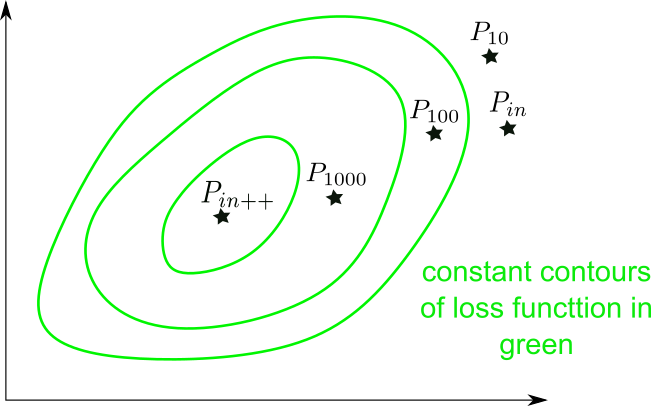
\includegraphics[width=3.2in]
{targeted-est/targeted-est.png}
\caption{
This figure portrays
the space of functions $\calh_\rvX$
as if it were the real plane $\RR^2$,
and the functional $\call[P, \haty=fixed]:\calh_\rvX
\rarrow\RR$
as if it were a real valued function on $\RR^2$.
It shows  the constant contours
of the loss functional $\call[P, \haty]$
at fixed $\haty$ in green.
$P_N$ for $N=10, 100, 1000$
represent empirical distributions.
The loss is non-negative and it equals
zero when $\eps=0$ and $P=P_{in++}$.
}
\label{fig-targeted-est}
\end{figure}

Note that function $\lam(X_\s)$ defined in Eq.(\ref{eq-loss-xi})
can be positive or negative. Hence,
 it can't be defined as the loss curve-fit,
because a loss curve-fit must be non-negative. However, it can be
defined as the derivative of a loss curve-fit. Suppose we define an $\eps\in\RR$
parameterized
family of probability distributions $P_\eps:val(\rvX)\rarrow [0,1]$,
and we expand the loss $\call[P_\eps, \haty]$
in powers of $\eps$:

\beq
\call[P_\eps, \haty] = \call[P_0, \haty]
+\eps \{\partial_\eps \call[P_\eps, \haty]\}_{\eps=0} + \calo(\eps^2)
\eeq
The parameter $\eps$ is called the {\bf fluctuation parameter}.
The function $\call[P_\eps, \haty]$ is obviously
not unique because all we know about it
is the value of its $\eps$ derivative
in the vicinity of $\eps=0$. Next we will pick a convenient
$\call[P_\eps, \haty]$ that satisfies

\beq
\call[P_\eps, \haty]\geq 0,\quad
\call[P_0, \haty]=0, \quad \partial_\eps \{\call[P_\eps, \haty]\}_{\eps=0}=0
\eeq


Use as loss curve-fit $\hatl$ the Cross Entropy
$CE(p\parallel q)$ for $p, q\in [0,1]$
\beq
\hatl = CE(p\parallel q)=-[p \ln q + (1-p) \ln(1- q)]
\eeq
$\hatl\geq 0$ and attains its minimum when $p=q$.
When $p=q$, it equals the entropy of $p$,
i.e., when $p=q$, $\hatl=-\sum_{x\in \bool} P(x)\ln P(x)= H(P)$,
where $P(0)=p, P(1)=1-p$.

For some $y\in\bool$ and $\eps\in\RR$,
make the following
substitutions
in the loss curve-fit $\hatl$
and call it $\hatl=\hatl(\beta, y, \haty, \eps)$.\footnote{To
agree with the TE literature,
we are using $\expit(x)$
(resp., $\logit(p)$) to denote
the sigmoid function (resp., log-odds function)
which we normally
denote in this book by
 $\smoid(x)$ (resp., $\lodds(p)$).}

\beq
p=y,
\quad
q= \expit[\logit(\haty) + \eps \beta ]
\eeq
Note that since $p=y$ is binary,
the minimum of this loss curve-fit is zero.


 Recall that in Section \ref{sec-smoid}, we proved that
 the derivative of $\expit(x)$ satisfies

\beq
\expit'(x) = \expit(x)[1-\expit(x)]
\;.
\eeq
Hence,

\begin{align}
\lim_{\eps\rarrow 0}\partial_\eps \hatl(\beta, y, \haty, \eps)
&=
\lim_{\eps\rarrow 0}
\left[-\;\frac{p}{q} + \frac{1-p}{1-q}\right]\partial_\eps q
\\
&=
\left[-\;\frac{y}{\haty} + \frac{1-y}{1-\haty}\right]
\lim_{\eps\rarrow 0}
\left\{
\begin{array}{l}
\expit[\logit(\haty) + \eps \beta ]
\\
*\left\{1-\expit[\logit(\haty) + \eps \beta ]\right\}
\beta
\end{array}
\right.
\\
&=
\left[-\;\frac{y}{\haty} + \frac{1-y}{1-\haty}\right]
\haty(1-\haty)\beta
\\
&=
\beta[\haty-y]
\end{align}

If we define $\hatl(X)$ by

\beq
\hatl(X) = \hatl
\left(
\begin{array}{l}
\beta=\frac{\Delta(d)}{P_{in++}(d|x)} ,
\\
y=y,
\\
\haty = \caly_{|d,x}[P_{in++}],
\\
\eps =\eps
\end{array}
\right)
\;,
\eeq
and $\call$ by

\beq
\call= \frac{1}{N}\sum_\s\hatl(X_\s) = P_N\cdot \hatl
\;,
\eeq
then

\beq
\left\{
\begin{array}{l}
\call=P_N\cdot \hatl\geq 0\\
\call_{\eps=0}=P_N\cdot
\hatl_{\eps=0}=0\\
\{\partial_\eps \call\}_{\eps=0}=
P_N\cdot\{\partial_\eps \hatl\}_{\eps=0} =0
\end{array}
\right.
\eeq


\section{$\Psi^{TMLE}$ in practice}
This section is based on Ref.\cite{hoff}.

In practice, one can calculate $\Psi^{TMLE}$
by performing the following steps.

Below, \qt{ML-fit} denotes a curve fitting
obtained using any valid machine learning method,
such as linear regression, a Neural Net, a
decision tree, etc. The TE software
often uses a \qt{Super-Learner}, a program that
 merges the results of multiple fits
obtained via various ML methods and also does cross validation.

Below , $\{(\s, d_\s, x_\s,\boxed{y_\s}):\s\in \Sigma\}$
represents a dataset. The dependent variable $y_\s$ is boxed,
the independent ones $d_\s,x_\s$ (a.k.a. covariates) aren't.

\begin{enumerate}
\item Find curve-fit $\haty(d,x)=\caly_{|d,x}$ of outcome $y$

\beq
\{(\s, d_\s, x_\s,\boxed{y_\s}):\s\in \Sigma\}\mlarr \haty(d,x)
\eeq

\item Estimate propensity $g(x)$

\beq
g(x)=P(\rvd=1|x)\approx
\frac{\sum_\s \delta(d_\s,1)\delta(x_\s, x)}
{\sum_\s \delta(x_\s, x)}
\eeq

\beq
P(d|x) = d g(x) + (1-d)[1-g(x)]
\eeq

\beq
\beta(d,x)=\frac{\Delta(d)}{P(d|x)}
\eeq

\item Estimate fluctuation parameter $\eps$

\beq
\eta(d,x) =
\underbrace{\logit[\haty(d, x)]}_
{\lam(d,x)}
 + \eps \beta(d, x)
\eeq

\beq
\{(\s, \lam(d_\s, x_\s),
\beta(d_\s, x_\s),\boxed{\eta(d_\s, x_\s)}:
\s\in \Sigma\}\mlarr \HAT{\eta}(d,x)
\eeq

\item Estimate ATE

\beq
ATE = \frac{1}{N} \sum_\s
\left\{
 \expit[ \HAT{\eta}(d=1,x_\s)]
 -\expit[ \HAT{\eta}(d=0,x_\s)]
 \right\}
\eeq

\end{enumerate}
